% !TeX root = ../Book1.tex
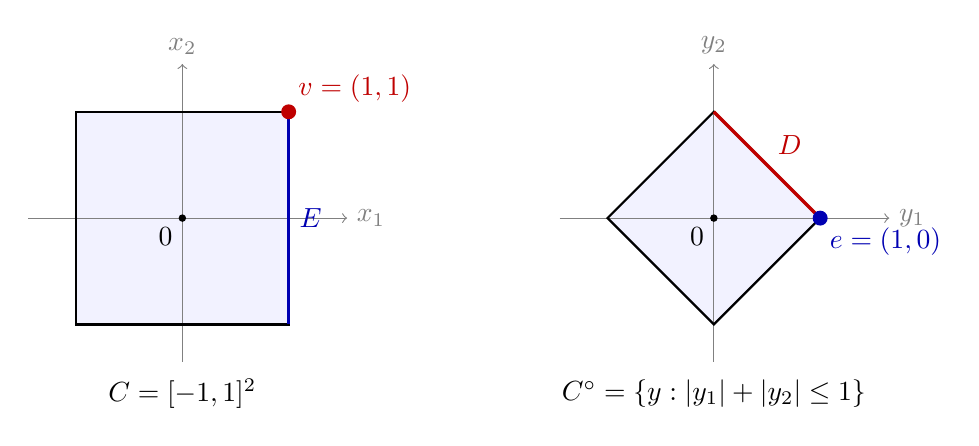
\begin{tikzpicture}[scale=1.35]
	\begin{scope}
		\fill[blue!5] (-1,-1) rectangle (1,1);
		\draw[->,gray] (-1.45,0)--(1.55,0) node[right] {\(x_1\)};
		\draw[->,gray] (0,-1.35)--(0,1.45) node[above] {\(x_2\)};
		\draw[thick] (-1,-1)--(1,-1)--(1,1)--(-1,1)--cycle;
		\draw[very thick,blue!70!black] (1,-1)--(1,1) node[midway,right] {\(E\)};
		\fill[red!75!black] (1,1) circle(2pt) node[above right] {\(v=(1,1)\)};
		\fill (0,0) circle(1pt) node[below left] {\(0\)};
		\node at (0,-1.65) {\(C=[-1,1]^2\)};
	\end{scope}
	\begin{scope}[xshift=5cm]
		\fill[blue!5] (1,0)--(0,1)--(-1,0)--(0,-1)--cycle;
		\draw[->,gray] (-1.45,0)--(1.65,0) node[right] {\(y_1\)};
		\draw[->,gray] (0,-1.35)--(0,1.45) node[above] {\(y_2\)};
		\draw[thick] (1,0)--(0,1)--(-1,0)--(0,-1)--cycle;
		\draw[very thick,red!75!black] (1,0)--(0,1) node[midway,above right] {\(D\)};
		\fill[blue!70!black] (1,0) circle(2pt) node[below right] {\(e=(1,0)\)};
		\fill (0,0) circle(1pt) node[below left] {\(0\)};
		\node at (0,-1.65) {\(C^\circ=\{y:|y_1|+|y_2|\le1\}\)};
	\end{scope}
\end{tikzpicture}
